\DocumentMetadata{}
\documentclass[sigconf, 10pt]{acmart}
\usepackage[compact]{titlesec}

\AtBeginDocument{%
  \providecommand\BibTeX{{%
    Bib\TeX}}}

\usepackage{hyperref}
\usepackage{longtable}
\usepackage{microtype}
\usepackage{enumitem}
\usepackage{xcolor}
\usepackage{amsmath,amsthm}
\usepackage{bbm}
\usepackage{subfigure}
\usepackage{graphicx}
\usepackage[font=small]{caption}
\usepackage{epstopdf}
\usepackage{algorithm}
\usepackage{tabularx}
\usepackage{multirow}
\usepackage[acronym,nogroupskip,nonumberlist,nopostdot]{glossaries}
\glsdisablehyper
\usepackage{xspace}
\usepackage{comment}
\usepackage{algorithm}
\usepackage[noend]{algorithmic}
\usepackage{makecell}
\usepackage{array}

\DeclareMathOperator*{\argmin}{arg\,min}
\DeclareMathOperator*{\argmax}{arg\,max}


\newcommand{\Expt}{\mathbb{E}}
\newcommand{\Prob}{\mathbb{P}}
\newcommand{\identity}{\mathbf{1}}
\newcommand{\Var}{\text{Var}}
\newcommand{\ttt}[1]{\texttt{#1}}
\newcommand{\cc}[1]{\mathcal{#1}}

\newcommand{\tblref}[1]{Table~\ref{#1}}
\newcommand{\equref}[1]{(\ref{#1})}
\newcommand{\figref}[1]{Fig. \ref{#1}}
\newcommand{\algref}[1]{Algorithm \ref{#1}}
\newcommand{\secref}[1]{Section \ref{#1}}
\newcommand{\appref}[1]{Appendix \ref{#1}~\cite{appendix}}
\newcommand{\lemmaref}[1]{Lemma \ref{#1}}
\newcommand{\defref}[1]{Definition \ref{#1}}
\newcommand{\exref}[1]{Example \ref{#1}}



\begin{document}

\acmYear{2024}\copyrightyear{2024}
\setcopyright{acmcopyright}
\acmConference[ACM MobiCom '25]{The 31th Annual International Conference On Mobile Computing And Networking}{November, 2025}{Hong Kong SAR, China}
\acmBooktitle{The 31th Annual International Conference On Mobile Computing And Networking (ACM MobiCom '25), November, 2025, Hong Kong SAR, China}
\acmDOI{10.1145/00000000}
\acmISBN{00000000}

\newcommand{\eg}{{\em e.g.}}

\newcolumntype{L}[1]{>{\raggedright\let\newline\\\arraybackslash\hspace{0pt}}m{#1}}
\newcolumntype{C}[1]{>{\centering\let\newline\\\arraybackslash\hspace{0pt}}m{#1}}
\newcolumntype{R}[1]{>{\raggedleft\let\newline\\\arraybackslash\hspace{0pt}}m{#1}}

\renewcommand{\cellalign}{vh}
\renewcommand{\theadalign}{vh}
\newcommand{\tsc}[1]{\textsuperscript{#1}}

\newtheorem*{takeaway*}{Takeaway}

\newcommand{\red}[1]{\textcolor{red}{#1}}

\newenvironment{sitemize}{
        \begin{list}{$\bullet$}{
                        \setlength{\itemsep}{2pt}
                        \setlength{\leftmargin}{1.2em}
                        \setlength{\topsep}{2pt plus 2pt minus 2pt}
                        \setlength{\parsep}{0.0cm}}
        }{\end{list}}

\newenvironment{senumerate}{
        \begin{list}{\arabic{enumi}.}{
                        \setlength\labelwidth{1.5em}
                        \setlength\leftmargin{1.5em}
                        \setlength{\topsep}{4pt plus 2pt minus 2pt}
                        \setlength\itemsep{0.0cm}
                        \usecounter{enumi}}
        }{\end{list}}

\settopmatter{authorsperrow=1}
\author{Changhan Ge}
\renewcommand{\shortauthors}{Changhan Ge}
\affiliation{
   \institution{The University of Texas at Austin, Austin, TX, USA}
   \institution{chge@utexas.edu}
   \country{}
   \city{}
}

\title{Petition to Adopt Year-specific Conference Logo Since ACM MobiCom 2025}

\newcommand{\wrt}{{\em w.r.t. }}
\newcommand{\para}[1]{\smallskip\noindent {\bf #1}}

\setlength{\abovecaptionskip}{0pt}
\setlength{\belowcaptionskip}{0pt}
\setlength{\abovedisplayshortskip}{0pt}
\setlength{\belowdisplayshortskip}{0pt}
\setlength{\textfloatsep}{0pt}

\begin{abstract}

\end{abstract}

\pagenumbering{gobble}

\keywords{MobiCom 2025, Branding}

\settopmatter{printfolios=true}

\maketitle

\section{Logo Design for MobiCom 2025}
As a part of the petition, we deign a preliminary logo for organizing committee's  reference. As shown in Fig. \ref{fig:logo}, the proposed logo for ACM MobiCom 2025 prominently incorporates a design that to reflect the cultural and symbolic elements of Hong Kong. There are two main designing elements described as follow:
\begin{itemize}[leftmargin=*]
	\item \textbf{Bauhinia Flower (Hong Kong’s Emblem):} The emblem of Hong Kong features a Bauhinia flower, which is often used to symbolize Hong Kong’s cultural significance and local heritage. We incorporate it by replacing the "0" in conference year "2025" with a modified version of the emblem. Specifically, we use pink and blush to recolor the originally maroon emblem, hence to reflect our young and vibrant community.
	
	\item \textbf{Victoria Harbour:} Victoria Harbour is one of Hong Kong’s most famous and iconic landmarks. The logo integrates elements that resemble the harbor, such as a wave-like pattern, a silhouette of ships, and the water itself, representing the flow of communication, global connectivity, and the idea of crossing boundaries. Victoria Harbour is also a hub of trade and technology, which aligns well with the themes of the conference focusing on mobile computing, networking, and beyond.
\end{itemize}
Note that, the silhouette of Hong Kong cityline  was designed with the help of ChatGPT, an LLM model owned and designed by OpenAI. The U.S. Copyright Office has already stated that works created by non-humans cannot be copyrighted \cite{copyright}. Hence there is no copyright issue involved in this logo design. The organizing committee and anyone who attend or involves in the conference can use the logo with no restrictions for non-profit purposes. We open-source the 

\begin{figure}[h]
	\centering
	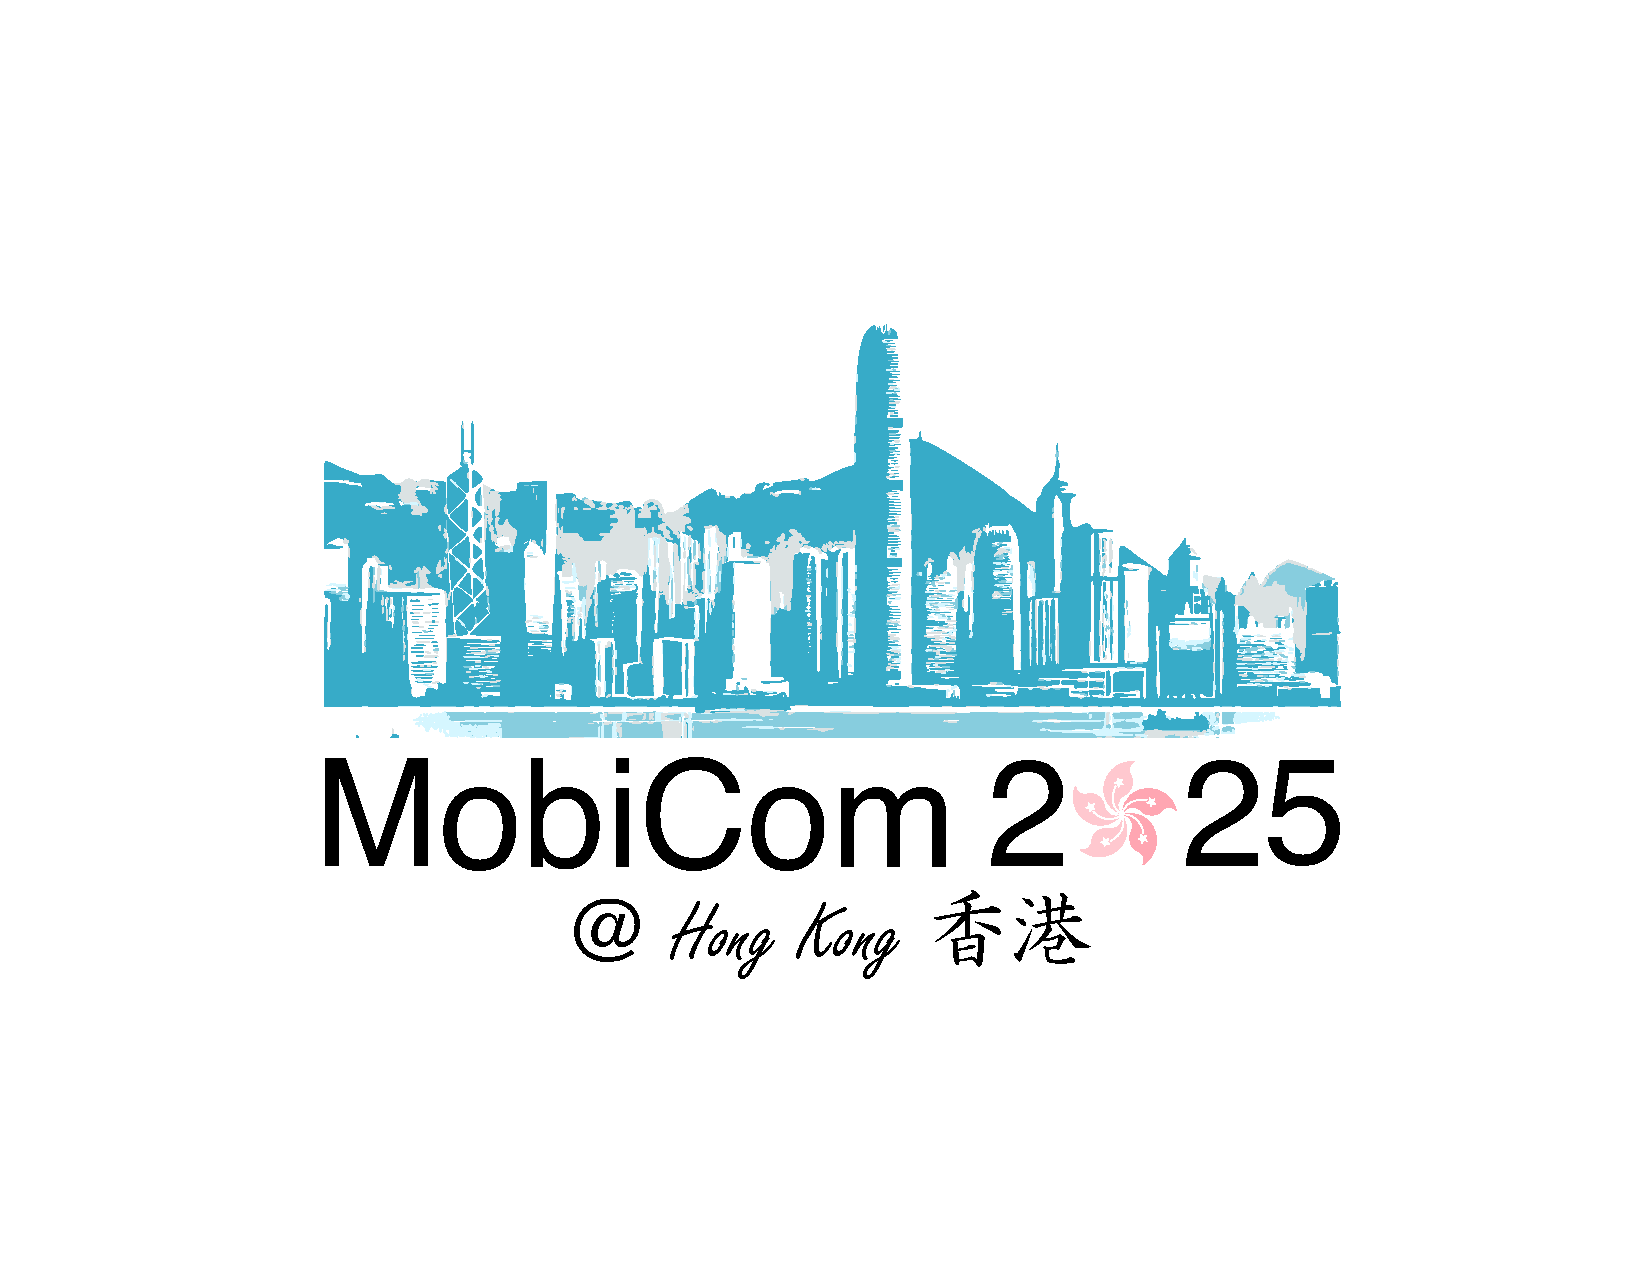
\includegraphics[width=\columnwidth, clip=true, trim=2cm 3cm 2cm 3cm]{../logo/mobicom25_logo.pdf}
	\caption{Proposed ACM MobiCom 2025 Logo}
	\label{fig:logo}
\end{figure}


\vspace{-3pt}
\section*{Acknowledgements}
\vspace{-3pt}
The author Changhan Ge @ UT Austin sincerely appreciates the help from ChatGPT, an LLM model owned and designed by OpenAI.

\appendix
\section{Logo Designs by Nearby Academic Community}
\begin{figure}[h]
	\centering
	
\includegraphics[width=\columnwidth]{./appendix/sigcomm25-logo.png}
	\caption{SIGCOMM 2025 Logo}
	\label{fig:sigcomm25logo}
\end{figure}

\begin{figure}[h]
	\centering
	
\includegraphics[width=\columnwidth]{./appendix/sigcomm24-logo.png}
	\caption{SIGCOMM 2024 Logo}
	\label{fig:sigcomm24logo}
\end{figure}

\begin{figure}[h]
	\centering
	
\includegraphics[width=\columnwidth]{./appendix/sigcomm23-logo.png}
	\caption{SIGCOMM 2023 Logo}
	\label{fig:sigcomm23logo}
\end{figure}

\begin{figure}[h]
	\centering
	
\includegraphics[width=\columnwidth]{./appendix/cvpr25-logo.jpg}
	\caption{CVPR 2025 Logo}
	\label{fig:cvpr25logo}
\end{figure}

\begin{figure}[h]
	\centering
	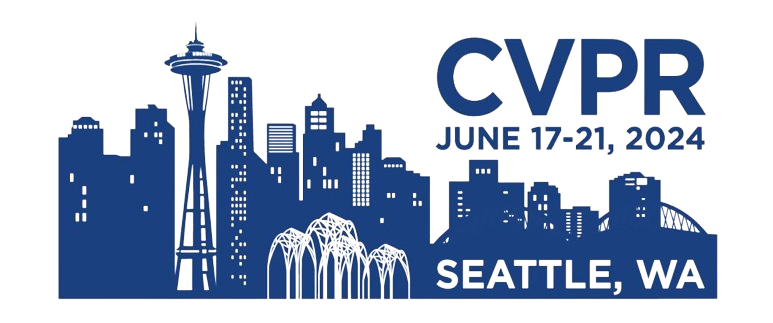
\includegraphics[width=\columnwidth]{./appendix/cvpr24-logo.png}
	\caption{CVPR 2024 Logo}
	\label{fig:cvpr24logo}
\end{figure}


\vspace{-3pt}
\bibliographystyle{ACM-Reference-Format}
\bibliography{reference}
\end{document}